\documentclass[10pt,twocolumn,a4paper]{article}

% -------------------------------------------------
% Language and encoding
% -------------------------------------------------
\usepackage[T1]{fontenc}
\usepackage{lmodern}
\usepackage[english]{babel}

% -------------------------------------------------
% Document format
% -------------------------------------------------
\usepackage[
    top=1.8cm,
    bottom=1.8cm,
    left=1.8cm,
    right=1.8cm,
    columnsep=0.7cm
]{geometry}

\usepackage{microtype}
\usepackage{parskip}

% -------------------------------------------------
% Mathematics
% -------------------------------------------------
\usepackage{amsmath}
\usepackage{amssymb}
\usepackage{bm}

% -------------------------------------------------
% Figures and tables
% -------------------------------------------------
\usepackage{graphicx}
\usepackage{subcaption}
\usepackage{booktabs}
\usepackage{siunitx}
\usepackage{placeins}

\usepackage{float}

% Normal spacing around figures
\setlength{\intextsep}{10pt plus 2pt minus 2pt}
\setlength{\textfloatsep}{10pt plus 2pt minus 2pt}
\setlength{\floatsep}{10pt plus 2pt minus 2pt}

\captionsetup[figure]{skip=5pt}

% -------------------------------------------------
% Links and references
% -------------------------------------------------
\usepackage[hidelinks]{hyperref}

% Folder containing generated figures
\graphicspath{{images/}}

% -------------------------------------------------
% Document information
% -------------------------------------------------
\title{
    \textbf{Artificial Potential Fields\\
    for\\
    Mobile Robot Navigation}
}

\author{
    Julio Quejido Barrera\\
    Humanoide Robotik\\
    Julio's Laboratories
}

\date{\today}

% =================================================
\begin{document}
% =================================================
\raggedbottom
\maketitle

\begin{abstract}
This project implements artificial potential fields for two-dimensional
mobile robot navigation. The target is modeled as an attractive potential
minimum, while circular obstacles generate repulsive potentials within a
finite influence distance. The robot evaluates the attractive and repulsive
forces at its current position, sums them, normalizes the resulting vector,
and advances in that direction using a discrete motion update. The main
implementation uses a quadratic attractive potential, which produces an
attractive force proportional to the distance from the goal. Conic and mixed
attractive potentials are also analyzed as alternative formulations. The
resulting scalar potential is represented as a three-dimensional surface and
a contour map, while the negative potential gradient is visualized as a
vector field. The experiment demonstrates obstacle avoidance without global
path planning, but also reveals characteristic limitations of the method,
including local equilibria and oscillation caused by normalized fixed-length
motion steps near the goal.
\end{abstract}

\section{Introduction}

Artificial potential fields provide a compact method for reactive robot
navigation. Instead of calculating a complete path in advance, the robot
interprets its environment as an artificial energy landscape. The goal forms
a low-potential region that attracts the robot, whereas obstacles form
high-potential regions that repel it.

At every simulation step, the robot calculates the local force produced by
this landscape. The attractive contribution points toward the goal and the
repulsive contributions point away from nearby obstacles. The sum of these
forces defines the instantaneous movement direction.

The method can be summarized as

\[
\begin{aligned}
    &\text{goal attraction}
    +
    \text{obstacle repulsion} \\
    &\hspace{2.5cm}\longrightarrow
    \text{local motion direction}.
\end{aligned}
\]

This project focuses on the quadratic attractive formulation. A second
implementation demonstrates the conic, or linear, attractive formulation,
while a mixed formulation is discussed as a compromise between both models.
The project also develops three complementary visualizations: the scalar
potential surface, a two-dimensional contour map, and the vector field of
normalized force directions.

\section{Theoretical Background}

\subsection{Robot, Goal, and Circular Obstacles}

The robot configuration is represented by the two-dimensional position

\[
    \mathbf{q}
    =
    \begin{bmatrix}
        x \\
        y
    \end{bmatrix},
\]

and the goal position by

\[
    \mathbf{q}_g
    =
    \begin{bmatrix}
        x_g \\
        y_g
    \end{bmatrix}.
\]

Each circular obstacle $i$ is described by its center

\[
    \mathbf{c}_i
    =
    \begin{bmatrix}
        c_{x,i} \\
        c_{y,i}
    \end{bmatrix}
\]

and radius $r_i$. This representation allows the repulsive interaction to
be based on the distance from the robot to the obstacle boundary rather than
only to its center.

\subsection{Potential and Force}

Let $U(\mathbf{q})$ be a scalar potential defined over the robot workspace.
The associated force is the negative gradient of that potential:

\begin{equation}
    \mathbf{F}(\mathbf{q})
    =
    -\nabla U(\mathbf{q}).
    \label{eq:negative_gradient}
\end{equation}

The gradient points in the direction of greatest potential increase.
Therefore, its negative points in the direction of steepest decrease. The
robot follows this descending direction locally at every iteration.

The total potential is decomposed into attractive and repulsive terms:

\begin{equation}
    U_{\mathrm{total}}(\mathbf{q})
    =
    U_{\mathrm{att}}(\mathbf{q})
    +
    \sum_i U_{\mathrm{rep},i}(\mathbf{q}).
    \label{eq:total_potential}
\end{equation}

Consequently,

\begin{equation}
    \mathbf{F}_{\mathrm{total}}
    =
    \mathbf{F}_{\mathrm{att}}
    +
    \sum_i \mathbf{F}_{\mathrm{rep},i}.
    \label{eq:total_force}
\end{equation}

\subsection{Quadratic Attractive Potential}

The main implementation uses the quadratic attractive potential

\begin{equation}
    U_{\mathrm{att}}(\mathbf{q})
    =
    \frac{1}{2}k_{\mathrm{att}}
    \left\|\mathbf{q}-\mathbf{q}_g\right\|^2,
    \label{eq:quadratic_potential}
\end{equation}

where $k_{\mathrm{att}}>0$ controls the strength of the attraction. The
potential is always non-negative and reaches its unique minimum at the goal:

\[
    \mathbf{q}=\mathbf{q}_g
    \quad\Rightarrow\quad
    U_{\mathrm{att}}=0.
\]

The expression is analogous to the potential energy of a linear spring. Its
gradient is

\[
    \nabla U_{\mathrm{att}}
    =
    k_{\mathrm{att}}(\mathbf{q}-\mathbf{q}_g),
\]

and therefore the attractive force is

\begin{equation}
    \mathbf{F}_{\mathrm{att}}
    =
    k_{\mathrm{att}}(\mathbf{q}_g-\mathbf{q}).
    \label{eq:quadratic_force}
\end{equation}

The force points directly from the robot toward the goal. Its magnitude is

\[
    \left\|\mathbf{F}_{\mathrm{att}}\right\|
    =
    k_{\mathrm{att}}
    \left\|\mathbf{q}_g-\mathbf{q}\right\|,
\]

so the unnormalized attractive force becomes stronger as the robot moves
farther from the goal and weaker as it approaches the minimum.

\subsection{Conic or Linear Attractive Potential}

A conic attractive landscape can be defined as

\begin{equation}
    U_{\mathrm{att}}^{\mathrm{lin}}(\mathbf{q})
    =
    k_{\mathrm{att}}d_g,
    \qquad
    d_g=\left\|\mathbf{q}-\mathbf{q}_g\right\|.
    \label{eq:linear_potential}
\end{equation}

For $d_g>0$, the associated force is

\begin{equation}
    \mathbf{F}_{\mathrm{att}}^{\mathrm{lin}}
    =
    k_{\mathrm{att}}
    \frac{\mathbf{q}_g-\mathbf{q}}
    {\left\|\mathbf{q}_g-\mathbf{q}\right\|}.
    \label{eq:linear_force}
\end{equation}

Its magnitude is approximately constant and equal to $k_{\mathrm{att}}$.
Unlike the quadratic formulation, the attraction does not grow without
bound as the distance increases. However, the conic potential is not smooth
at the goal. The separate linear implementation therefore suppresses the
attractive force inside a small neighborhood of the goal.

The linear demonstration also uses a different obstacle influence distance
from the quadratic experiment. Its trajectory should consequently not be
interpreted as a comparison caused exclusively by the attractive potential.

\subsection{Mixed Attractive Potential}

A mixed formulation combines the smooth behavior of the quadratic potential
near the target with a bounded attractive force far from it. Let $d^*>0$ be
a switching distance. The potential can be defined as

\begin{equation}
U_{\mathrm{att}}^{\mathrm{mix}}(d_g)
=
\begin{cases}
\dfrac{1}{2}k_{\mathrm{att}}d_g^2,
& d_g\leq d^*, \\

k_{\mathrm{att}}d^*
\left(d_g-\dfrac{1}{2}d^*\right),
& d_g>d^*.
\end{cases}
\label{eq:mixed_potential}
\end{equation}

The corresponding attractive force is

\begin{equation}
\mathbf{F}_{\mathrm{att}}^{\mathrm{mix}}
=
\begin{cases}

k_{\mathrm{att}}(\mathbf{q}_g-\mathbf{q}),
& d_g\leq d^*, \\

k_{\mathrm{att}}d^*
\dfrac{\mathbf{q}_g-\mathbf{q}}{d_g},
& d_g>d^*.
\end{cases}
\label{eq:mixed_force}
\end{equation}

Thus, the force is proportional to distance near the goal and has bounded
magnitude $k_{\mathrm{att}}d^*$ farther away. This formulation is discussed
theoretically but is not implemented in the supplied experiment.

\begin{table}[htbp]
\centering
\caption{Comparison of attractive potential models.}
\label{tab:attractive_models}
\small
\begin{tabular}{lcc}
\toprule
\textbf{Model} & \textbf{Potential} & \textbf{Force} \\
\midrule
Quadratic & $d_g^2$ & $\propto d_g$ \\
Conic & $d_g$ & constant \\
Mixed & quadratic/linear & proportional/bounded \\
\bottomrule
\end{tabular}
\end{table}

\subsection{Distance to an Obstacle Boundary}

For obstacle $i$, the distance from the robot to its center is

\[
    d_{\mathrm{center},i}
    =
    \left\|\mathbf{q}-\mathbf{c}_i\right\|.
\]

Because the obstacle has radius $r_i$, the relevant clearance is

\begin{equation}
    d_i
    =
    \left\|\mathbf{q}-\mathbf{c}_i\right\|-r_i.
    \label{eq:clearance}
\end{equation}

The sign of this quantity has a direct geometric meaning:

\[
\begin{aligned}
    d_i>0 &\quad\Rightarrow\quad \text{robot outside the obstacle},\\
    d_i=0 &\quad\Rightarrow\quad \text{robot on the boundary},\\
    d_i<0 &\quad\Rightarrow\quad \text{robot inside the obstacle}.
\end{aligned}
\]

\subsection{Repulsive Potential}

Repulsion is active only inside a finite influence distance $\rho_0$. To
avoid division by zero or excessively large numerical values, the clearance
used in reciprocal terms is bounded from below:

\begin{equation}
    \bar d_i
    =
    \max(d_i,\varepsilon).
    \label{eq:safe_distance}
\end{equation}

The repulsive potential implemented for obstacle $i$ is

\begin{equation}
U_{\mathrm{rep},i}(\mathbf{q})
=
\begin{cases}
\dfrac{1}{2}k_{\mathrm{rep}}
\left(
\dfrac{1}{\bar d_i}
-
\dfrac{1}{\rho_0}
\right)^2,
& d_i\leq\rho_0,\\[3mm]
0,
& d_i>\rho_0.
\end{cases}
\label{eq:repulsive_potential}
\end{equation}

At $d_i=\rho_0$, the active expression becomes zero. As the robot
approaches the obstacle boundary, $1/\bar d_i$ grows rapidly and the
potential forms a steep barrier.

\subsection{Repulsive Force Derivation}

Inside the influence region, define

\[
    s(d_i)
    =
    \frac{1}{d_i}-\frac{1}{\rho_0}.
\]

Ignoring the numerical lower bound temporarily, differentiation gives

\[
    \frac{d}{d d_i}\left(\frac{1}{d_i}\right)
    =
    -\frac{1}{d_i^2}.
\]

Therefore,

\[
    \frac{dU_{\mathrm{rep},i}}{d d_i}
    =
    -k_{\mathrm{rep}}
    \left(
    \frac{1}{d_i}-\frac{1}{\rho_0}
    \right)
    \frac{1}{d_i^2}.
\]

The unit vector pointing from the obstacle center toward the robot is

\begin{equation}
    \hat{\mathbf{u}}_i
    =
    \frac{\mathbf{q}-\mathbf{c}_i}
    {\left\|\mathbf{q}-\mathbf{c}_i\right\|}.
    \label{eq:repulsive_direction}
\end{equation}

Using the safeguarded clearance from Equation~\eqref{eq:safe_distance},
the implemented repulsive force is

\begin{equation}
\mathbf{F}_{\mathrm{rep},i}
=
\begin{cases}

k_{\mathrm{rep}}
\left(
\dfrac{1}{\bar d_i}
-
\dfrac{1}{\rho_0}
\right)
\dfrac{1}{\bar d_i^2}
\hat{\mathbf{u}}_i,
& d_i\leq\rho_0,\\[3mm]

\mathbf{0},
& d_i>\rho_0.
\end{cases}
\label{eq:repulsive_force}
\end{equation}

The factor $1/\bar d_i^2$ appears from differentiating the reciprocal
distance. It makes the repulsion increase sharply near the obstacle.
Contributions from all obstacles are added to form the total repulsive
force.

\subsection{Normalized Total Force and Robot Motion}

After adding attractive and repulsive contributions, the experiment
normalizes the total force:

\begin{equation}
    \hat{\mathbf{F}}_{\mathrm{total}}
    =
    \frac{\mathbf{F}_{\mathrm{total}}}
    {\left\|\mathbf{F}_{\mathrm{total}}\right\|}.
    \label{eq:normalized_force}
\end{equation}

If the total force is the zero vector, the normalization routine returns the
zero vector. The robot position is then updated using

\begin{equation}
    \mathbf{q}_{t+1}
    =
    \mathbf{q}_t
    +
    v\,\hat{\mathbf{F}}_{\mathrm{total}}\Delta t.
    \label{eq:motion_update}
\end{equation}

Normalizing the force means that only its direction is used for motion. With
$v=0.2$ and $\Delta t=1$, every nonzero update has length

\[
    \left\|\mathbf{q}_{t+1}-\mathbf{q}_t\right\|=0.2.
\]

This produces a constant translational step even when the unnormalized
force becomes small near the goal.

\subsection{Potential Landscape and Force Field}

The scalar potential and the vector force field describe different aspects
of the same navigation method:

\begin{itemize}
    \item the three-dimensional surface shows the complete energy landscape;
    \item the contour map shows equal-potential curves viewed from above;
    \item the vector field shows the local direction of
    $-\nabla U_{\mathrm{total}}$;
    \item the trajectory shows the positions actually visited by the robot.
\end{itemize}

In the vector-field visualization, every force vector is normalized before
being plotted. The arrows therefore show direction rather than relative
force magnitude. In the contour visualization, high potential values are
clipped for display so that the obstacle peaks do not dominate the complete
color scale.

\subsection{Local Minima and Other Limitations}

A local equilibrium occurs when

\begin{equation}
    \mathbf{F}_{\mathrm{total}}(\mathbf{q})
    =
    \mathbf{0},
    \qquad
    \mathbf{q}\neq\mathbf{q}_g.
    \label{eq:local_minimum}
\end{equation}

At such a point, attractive and repulsive forces cancel. Because the method
uses only local information, it cannot determine that another route around
the obstacles would eventually reach the goal. Narrow passages, symmetric
obstacle arrangements, and strong repulsive gains can also produce
oscillations or excessive detours.

The normalized motion update introduces an additional numerical limitation.
The quadratic attractive force becomes small near the goal, but
normalization removes this decrease in magnitude. Unless the fixed step
happens to enter the tolerance region, the robot may pass across the goal
and oscillate around it. A distance-dependent speed or an unnormalized
force update would provide smoother convergence.

\section{Experimental Configuration}

The quadratic potential-field experiment begins at

\[
    \mathbf{q}_0
    =
    \begin{bmatrix}
        0 \\
        3
    \end{bmatrix},
    \qquad
    \mathbf{q}_g
    =
    \begin{bmatrix}
        6 \\
        4
    \end{bmatrix}.
\]

Four circular obstacles are included in the environment. Each obstacle
is defined by its center $\mathbf{c}_i$ and radius $r_i$, as shown in
Table~\ref{tab:obstacles}.

\begin{table}[htbp]
\centering
\caption{Circular obstacle configuration.}
\label{tab:obstacles}
\begin{tabular}{ccc}
\toprule
\textbf{Obstacle} &
\textbf{Center} $\mathbf{c}_i$ &
\textbf{Radius} $r_i$ \\
\midrule
$O_1$ & $[3,\,3]^T$ & $0.3$ \\
$O_2$ & $[6,\,1]^T$ & $0.5$ \\
$O_3$ & $[3,\,5]^T$ & $0.5$ \\
$O_4$ & $[4,\,4]^T$ & $0.1$ \\
\bottomrule
\end{tabular}
\end{table}

The parameters used for the attractive and repulsive potential fields
and for the discrete robot motion are listed in
Table~\ref{tab:parameters}.

\begin{table}[htbp]
\centering
\caption{Quadratic potential-field parameters.}
\label{tab:parameters}
\begin{tabular}{lll}
\toprule
\textbf{Parameter} &
\textbf{Symbol} &
\textbf{Value} \\
\midrule
Attractive gain &
$k_{\mathrm{att}}$ &
$2.5$ \\

Repulsive gain &
$k_{\mathrm{rep}}$ &
$1.0$ \\

Influence distance &
$\rho_0$ &
$0.5$ \\

Minimum clearance &
$\varepsilon$ &
$0.08$ \\

Motion speed &
$v$ &
$0.2$ \\

Time step &
$\Delta t$ &
$1.0$ \\

Goal tolerance &
$d_{\mathrm{tol}}$ &
$0.01$ \\

Maximum steps &
$N_{\max}$ &
$10000$ \\
\bottomrule
\end{tabular}
\end{table}

At each iteration, the attractive force and the repulsive contributions
of all obstacles are calculated at the current robot position. The
resulting total force is normalized and used in the discrete motion
update given by Equation~\eqref{eq:motion_update}.

The simulation terminates when the distance between the robot and the
goal satisfies

\[
    \left\|
        \mathbf{q}_t-\mathbf{q}_g
    \right\|
    \leq
    d_{\mathrm{tol}},
\]

or when the maximum number of iterations $N_{\max}$ is reached.

For the potential-field visualizations, the scalar potential is evaluated
over a two-dimensional rectangular grid defined by

\[
    -1 \leq x \leq 8,
    \qquad
    -1 \leq y \leq 7.
\]

The grid contains $150$ samples along each coordinate axis. A separate
$25\times25$ grid is used for the vector-field representation, where
the total force is evaluated and normalized at every grid point.

\section{Results and Discussion}

\subsection{Three-Dimensional Potential Landscape}

Figure~\ref{fig:potential_surface_3d} represents the total artificial
potential as a three-dimensional surface. The horizontal axes correspond to
the position coordinates $x$ and $y$, while the vertical axis represents the
total potential

\[
    U_{\mathrm{total}}(\mathbf{q})
    =
    U_{\mathrm{att}}(\mathbf{q})
    +
    \sum_i U_{\mathrm{rep},i}(\mathbf{q}).
\]

The quadratic attractive potential produces a broad bowl-shaped surface
centered at the goal. Because

\[
    U_{\mathrm{att}}(\mathbf{q})
    =
    \frac{1}{2}
    k_{\mathrm{att}}
    \left\|
        \mathbf{q}-\mathbf{q}_g
    \right\|^2,
\]

the potential increases quadratically with the distance from the target.
The goal therefore appears at the bottom of the attractive basin, where the
attractive potential reaches its minimum value.

The repulsive potentials generate steep peaks around the circular
obstacles. Their rapid growth is caused by the reciprocal-clearance term

\[
    \left(
        \frac{1}{\bar d_i}
        -
        \frac{1}{\rho_0}
    \right)^2,
\]

which becomes large as the robot approaches an obstacle boundary. The
protected clearance

\[
    \bar d_i
    =
    \max(d_i,\varepsilon)
\]

prevents division by zero and limits the numerical value of the peaks,
although they remain considerably steeper than the surrounding attractive
surface.

The red curve represents the simulated trajectory evaluated on the
potential surface. It begins at

\[
    \mathbf{q}_0
    =
    \begin{bmatrix}
        0\\
        3
    \end{bmatrix}
\]

and descends toward the goal at

\[
    \mathbf{q}_g
    =
    \begin{bmatrix}
        6\\
        4
    \end{bmatrix}.
\]

For visual clarity, the trajectory is drawn with a small vertical offset
above the surface. This offset changes only the graphical representation and
does not modify the calculated potential or the robot motion.

The path does not follow a perfectly straight descent. When the robot enters
the repulsive influence region of an obstacle, the local slope of the total
potential changes. The repulsive gradient modifies the direction of descent,
causing the trajectory to move around the corresponding potential peak
before continuing toward the goal.

\begin{figure}[htbp]
    \centering
    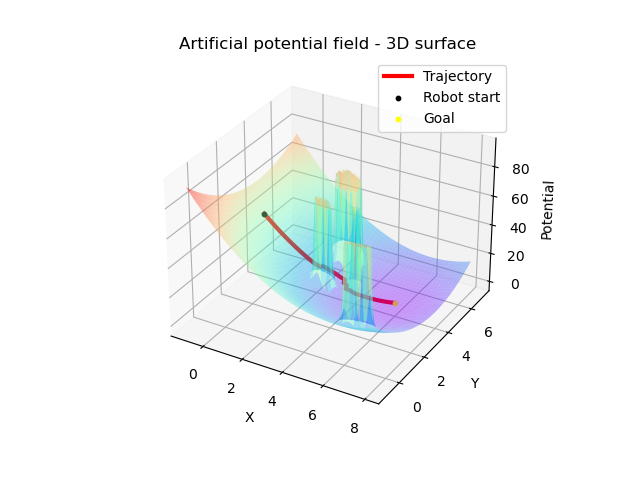
\includegraphics[width=\columnwidth]{Figure_1_1.png}
    \caption{Three-dimensional total-potential surface. The quadratic
    attractive potential forms a broad basin around the goal, while the
    repulsive potentials generate steep peaks near the circular obstacles.
    The red curve shows the simulated robot trajectory.}
    \label{fig:potential_surface_3d}
\end{figure}


\subsection{Contour Map and Robot Trajectory}

Figure~\ref{fig:potential_contour_map} presents the same scalar potential
from a top-down perspective. Every contour line connects points having the
same total-potential value. The color distribution therefore provides a
two-dimensional representation of the energy landscape shown in
Figure~\ref{fig:potential_surface_3d}.

Low-potential regions are concentrated around the goal, whereas higher
potential values appear farther from the target and around the obstacles.
The approximately circular contours surrounding the goal originate mainly
from the quadratic attractive term. In the absence of obstacles, these
contours would be concentric circles centered at $\mathbf{q}_g$.

Near an obstacle, the contour lines become strongly deformed and closely
spaced. A high density of contour lines indicates a steep potential
gradient. Consequently, these regions generate a strong change in the
direction of the total force.

For visual readability, the displayed potential is limited to

\[
    0
    \leq
    U_{\mathrm{plot}}
    \leq
    100.
\]

This clipping affects only the color scale. The complete, unclipped
potential is still used to calculate the forces and the robot trajectory.
Without this graphical limit, the very large repulsive values close to the
obstacle boundaries would dominate the color map and make the attractive
basin difficult to observe.

The circles drawn in the figure represent the physical obstacle boundaries.
However, the repulsive force begins before the robot reaches these
boundaries. Since the clearance is

\[
    d_i
    =
    \left\|
        \mathbf{q}-\mathbf{c}_i
    \right\|
    -
    r_i,
\]

and repulsion is active when

\[
    d_i
    \leq
    \rho_0,
\]

the effective distance of influence measured from the obstacle center is

\[
    R_{\mathrm{influence},i}
    =
    r_i+\rho_0.
\]

For the current experiment, the influence distances from the obstacle
centers are therefore

\[
\begin{aligned}
    R_{\mathrm{influence},1} &= 0.3+0.5=0.8,\\
    R_{\mathrm{influence},2} &= 0.5+0.5=1.0,\\
    R_{\mathrm{influence},3} &= 0.5+0.5=1.0,\\
    R_{\mathrm{influence},4} &= 0.1+0.5=0.6.
\end{aligned}
\]

The robot initially moves approximately toward the goal under the dominant
attractive force. Obstacle $O_1$ lies close to this direct route. As the
robot enters its influence region, the repulsive contribution bends the
trajectory upward and prevents collision with the obstacle.

After passing $O_1$, the robot again turns toward the goal. A second local
deviation appears near the smaller obstacle $O_4$. Although its physical
radius is only $0.1$, it still generates repulsion within a clearance of
$\rho_0=0.5$. The trajectory passes below this obstacle and subsequently
returns toward the attractive minimum.

Obstacles $O_2$ and $O_3$ remain visible in the potential map, but they do
not significantly modify the observed path because the trajectory does not
enter their corresponding influence regions. The final robot marker lies
within the goal tolerance and is therefore almost completely covered by the
goal marker in the figure.

\begin{figure}[H]
    \centering
    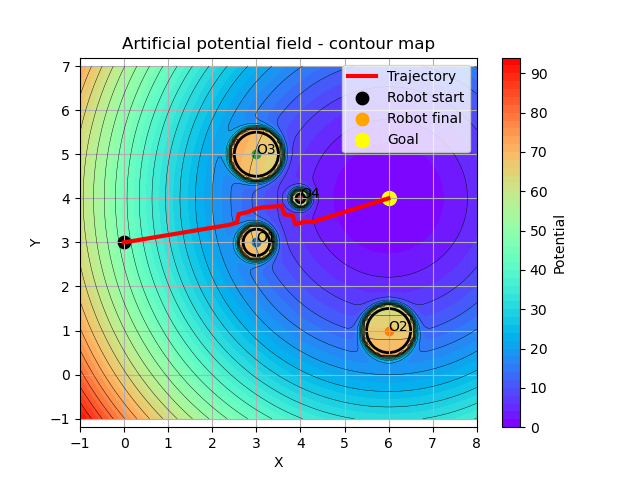
\includegraphics[width=\columnwidth]{Figure_1_2.png}
    \caption{Contour map of the total potential and the resulting robot
    trajectory. Closely spaced contour lines indicate steep potential
    gradients near obstacle boundaries. Potential values are clipped only
    for graphical readability.}
    \label{fig:potential_contour_map}
\end{figure}

\FloatBarrier

\subsection{Normalized Force Vector Field}

Figure~\ref{fig:potential_vector_field} shows the direction of the total
artificial force at different positions in the workspace. At every sampled
point, the attractive and repulsive contributions are added:

\[
    \mathbf{F}_{\mathrm{total}}
    =
    \mathbf{F}_{\mathrm{att}}
    +
    \sum_i \mathbf{F}_{\mathrm{rep},i}.
\]

The plotted vector is then normalized:

\[
    \hat{\mathbf{F}}_{\mathrm{total}}
    =
    \frac{
        \mathbf{F}_{\mathrm{total}}
    }{
        \left\|
            \mathbf{F}_{\mathrm{total}}
        \right\|
    }.
\]

As a result, the arrows represent only the local motion direction. Their
displayed lengths must not be interpreted as the magnitude of the actual
force. A weak attractive force and a very strong repulsive force can appear
with similar arrow lengths after normalization.

Far from all obstacles, the repulsive contribution is zero and the arrows
point mainly toward the goal:

\[
    \mathbf{F}_{\mathrm{total}}
    \approx
    \mathbf{F}_{\mathrm{att}}.
\]

The vector field therefore exhibits a general convergence pattern toward
$\mathbf{q}_g$. This behavior is especially clear in the right-hand region
of the map, where the arrows point toward the target from different
directions.

Near obstacle boundaries, the repulsive force changes the orientation of
the vectors. The arrows rotate away from the obstacle centers and create
local flows around the circular regions. Around $O_1$, the force field
redirects the robot upward. Around $O_4$, the field produces a second
deflection that guides the robot below the obstacle.

The simulated trajectory follows these local force directions closely. Its
shape can therefore be interpreted directly from the surrounding arrows:

\[
    \text{local force direction}
    \quad\longrightarrow\quad
    \text{next robot displacement}.
\]

Because the same normalized force is used in the discrete motion update,

\[
    \mathbf{q}_{t+1}
    =
    \mathbf{q}_t
    +
    v
    \hat{\mathbf{F}}_{\mathrm{total}}
    \Delta t,
\]

each nonzero displacement has the fixed length

\[
    v\Delta t
    =
    0.2.
\]

The small angular changes visible in the trajectory near the obstacles are
therefore produced by the combination of a fixed motion step and rapidly
changing repulsive directions.

Some arrows are also displayed inside the circular obstacles because the
force field is evaluated over the complete rectangular grid. These vectors
are a mathematical extension of the field used for visualization; positions
inside the obstacles are not valid robot configurations and are not visited
by the simulated trajectory.

\begin{figure}[htbp]
    \centering
    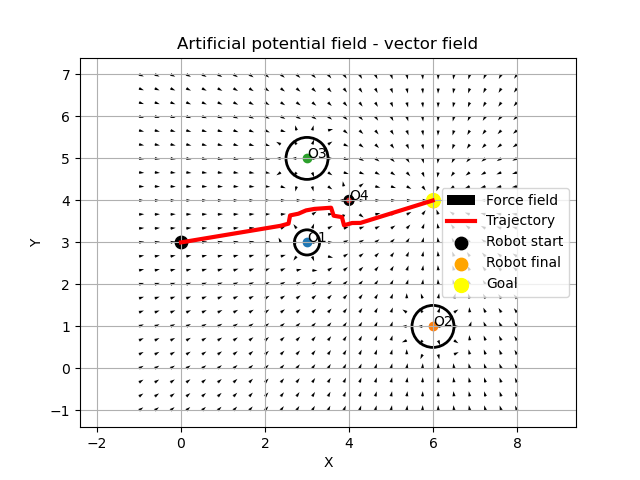
\includegraphics[width=\columnwidth]{Figure_1_3.png}
    \caption{Normalized total-force vector field and simulated trajectory.
    Far from the obstacles, the arrows point mainly toward the goal. Near
    obstacle boundaries, the repulsive terms redirect the field away from
    the obstacle centers.}
    \label{fig:potential_vector_field}
\end{figure}


\subsection{Combined Interpretation}

The three representations describe different aspects of the same navigation
process. The three-dimensional surface represents the artificial energy
landscape, the contour map shows the spatial distribution of equal-potential
regions, and the vector field shows the local direction of steepest
potential decrease.

Their relationship can be summarized as

\[
\begin{aligned}
    \text{potential surface}
    &\longrightarrow
    \text{energy landscape},\\
    \text{contour map}
    &\longrightarrow
    \text{top-down potential distribution},\\
    \text{vector field}
    &\longrightarrow
    \text{local movement direction},\\
    \text{trajectory}
    &\longrightarrow
    \text{positions actually visited}.
\end{aligned}
\]

The experiment demonstrates that the robot can reach the target while
avoiding the obstacles without calculating a complete path in advance. At
each iteration, it uses only the total force at its current position.
Consequently, the final route emerges from repeated local decisions rather
than from a global path-planning algorithm.

\subsection{Influence of the Attractive Gain}

The attractive gain determines the strength of the force directed toward
the goal:

\begin{equation}
    \mathbf{F}_{\mathrm{att}}
    =
    k_{\mathrm{att}}
    \left(
        \mathbf{q}_g-\mathbf{q}
    \right).
\end{equation}

It also scales the quadratic attractive potential:

\begin{equation}
    U_{\mathrm{att}}(\mathbf{q})
    =
    \frac{1}{2}
    k_{\mathrm{att}}
    \left\|
        \mathbf{q}-\mathbf{q}_g
    \right\|^2.
\end{equation}

Since the total force is normalized before updating the robot position,
changing $k_{\mathrm{att}}$ does not modify the displacement length
directly. Instead, it changes the balance between attraction and
repulsion and therefore modifies the direction of motion.

\subsubsection{Low Attractive Gain}

For

\[
    k_{\mathrm{att}}=0.5,
\]

the attractive contribution is relatively weak compared with the
repulsive forces. The robot is strongly redirected near obstacles
$O_1$ and $O_4$, producing a larger deviation from the direct path and
visible oscillations between both obstacles.

The three-dimensional surface also shows a shallower attractive basin.
Therefore, the repulsive peaks have a stronger relative influence on
the total potential.

\begin{figure}[H]
    \centering
    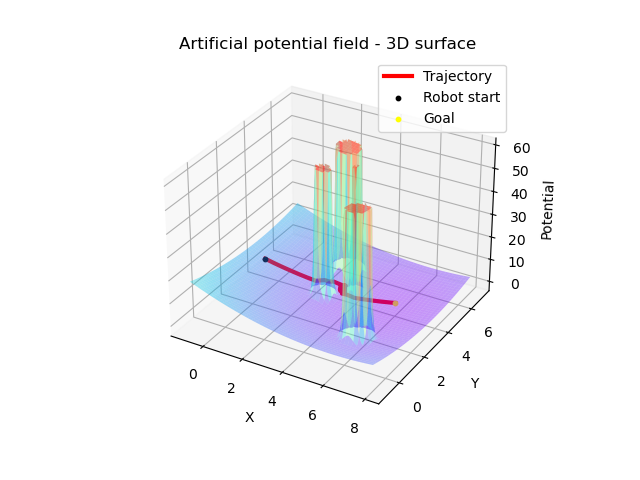
\includegraphics[width=\columnwidth]{Figure_3_1.png}
    \caption{Potential surface for a low attractive gain,
    $k_{\mathrm{att}}=0.5$.}
    \label{fig:katt_low_surface}
\end{figure}

\begin{figure}[H]
    \centering
    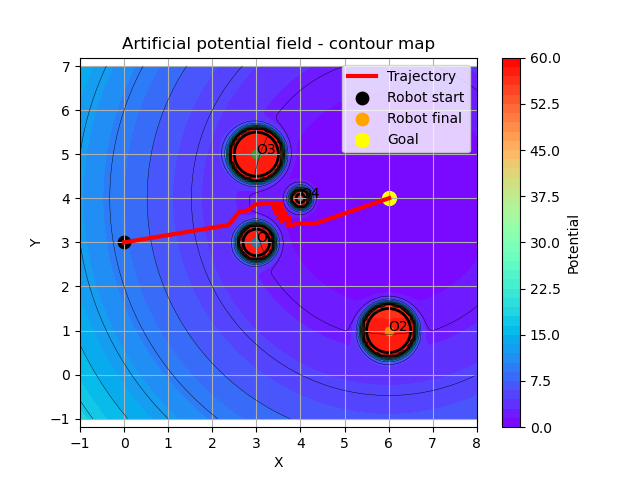
\includegraphics[width=\columnwidth]{Figure_3_2.png}
    \caption{Contour map and robot trajectory for
    $k_{\mathrm{att}}=0.5$. The obstacle potentials have a strong
    influence relative to the shallow attractive basin.}
    \label{fig:katt_low_contour}
\end{figure}

\begin{figure}[H]
    \centering
    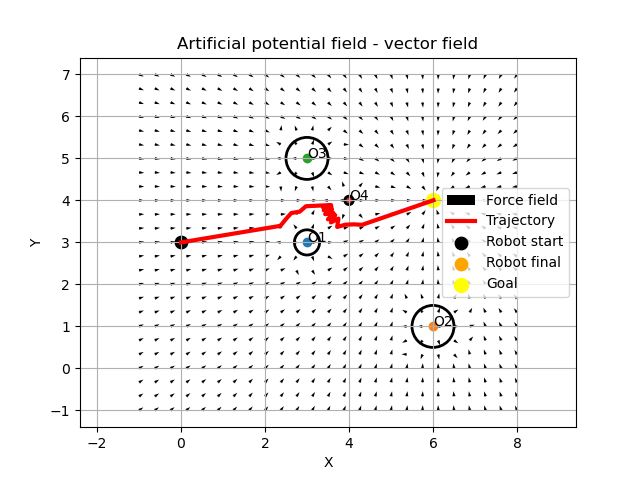
\includegraphics[width=\columnwidth]{Figure_3_3.png}
    \caption{Normalized force field for $k_{\mathrm{att}}=0.5$.
    Strong changes in direction appear near $O_1$ and $O_4$.}
    \label{fig:katt_low_vector}
\end{figure}


\subsubsection{High Attractive Gain}

For

\[
    k_{\mathrm{att}}=10,
\]

the attractive force dominates a larger part of the workspace. The
robot follows a smoother and more direct trajectory toward the goal,
while the obstacles cause only local deviations.

The quadratic attractive potential also grows more rapidly with
distance, producing a much steeper attractive basin. Nevertheless, an
excessively large value of $k_{\mathrm{att}}$ reduces the relative
influence of the repulsive forces and may cause the robot to pass too
close to an obstacle.

\begin{figure}[H]
    \centering
    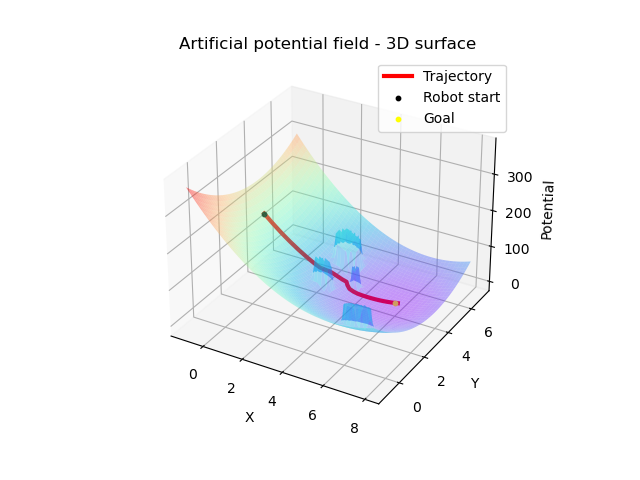
\includegraphics[width=\columnwidth]{Figure_2_1.png}
    \caption{Potential surface for a high attractive gain,
    $k_{\mathrm{att}}=10$.}
    \label{fig:katt_high_surface}
\end{figure}

\begin{figure}[H]
    \centering
    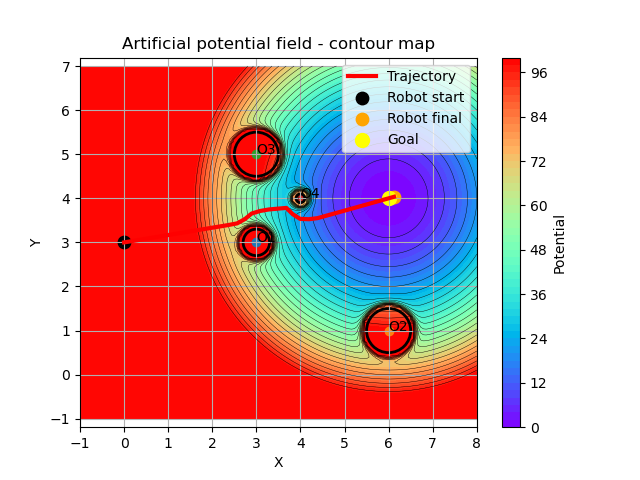
\includegraphics[width=\columnwidth]{Figure_2_2.png}
    \caption{Contour map and robot trajectory for
    $k_{\mathrm{att}}=10$. The steep attractive basin dominates most
    of the workspace.}
    \label{fig:katt_high_contour}
\end{figure}

\begin{figure}[H]
    \centering
    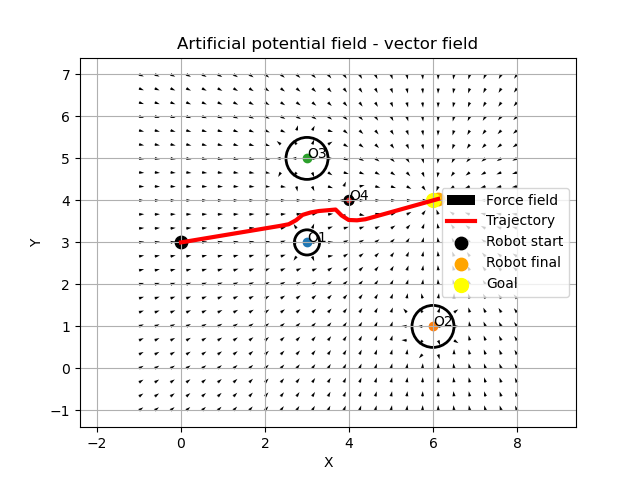
\includegraphics[width=\columnwidth]{Figure_2_3.png}
    \caption{Normalized force field for $k_{\mathrm{att}}=10$.
    Most vectors point strongly toward the goal, except close to the
    obstacles.}
    \label{fig:katt_high_vector}
\end{figure}

The comparison can be summarized as

\[
\begin{aligned}
    k_{\mathrm{att}}\ \text{small}
    &\Rightarrow
    \text{greater relative repulsive influence},\\
    k_{\mathrm{att}}\ \text{large}
    &\Rightarrow
    \text{greater attractive influence}.
\end{aligned}
\]

A suitable value must preserve sufficient attraction toward the goal
without making the obstacle-avoidance contribution too weak.

\FloatBarrier

\subsection{Influence of the Repulsive Gain}

The repulsive gain scales the obstacle potential and the corresponding
repulsive force:

\begin{equation}
    U_{\mathrm{rep},i}
    =
    \frac{1}{2}
    k_{\mathrm{rep}}
    \left(
        \frac{1}{\bar d_i}
        -
        \frac{1}{\rho_0}
    \right)^2,
\end{equation}

\begin{equation}
    \mathbf{F}_{\mathrm{rep},i}
    =
    k_{\mathrm{rep}}
    \left(
        \frac{1}{\bar d_i}
        -
        \frac{1}{\rho_0}
    \right)
    \frac{1}{\bar d_i^2}
    \hat{\mathbf{u}}_i.
\end{equation}

The repulsive gain was increased from its reference value
$k_{\mathrm{rep}}=1$ to

\[
    k_{\mathrm{rep}}=5.
\]

The influence distance remains unchanged at $\rho_0=0.5$. Therefore,
increasing $k_{\mathrm{rep}}$ does not enlarge the region in which an
obstacle is detected by the potential field. It only increases the
strength of the repulsion inside that region.

The stronger repulsive contribution produces higher potential peaks
around the obstacles. When the robot approaches $O_1$ and $O_4$, the
repulsive forces dominate the local direction of the total field and
cause a stronger deviation from the direct path.

Because the total force is normalized before the position update,
increasing $k_{\mathrm{rep}}$ does not increase the length of each motion
step. Instead, it changes the direction of motion by increasing the
relative importance of obstacle avoidance.

\begin{figure}[H]
    \centering
    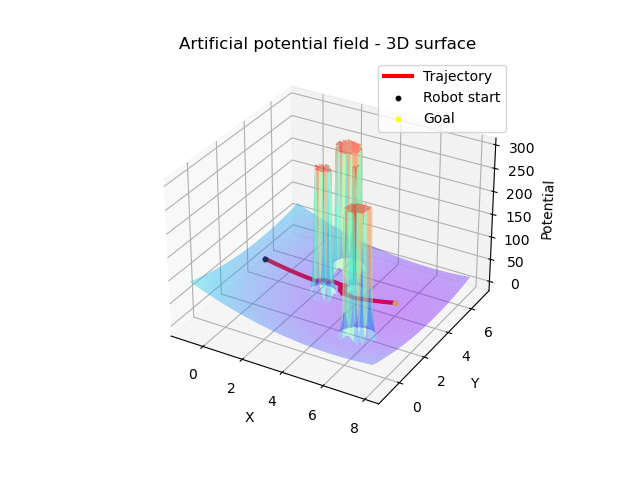
\includegraphics[width=\columnwidth]{Figure_4_1.png}
    \caption{Potential surface for an increased repulsive gain,
    $k_{\mathrm{rep}}=5$. The obstacle peaks become more dominant
    relative to the attractive basin.}
    \label{fig:krep_high_surface}
\end{figure}

\begin{figure}[H]
    \centering
    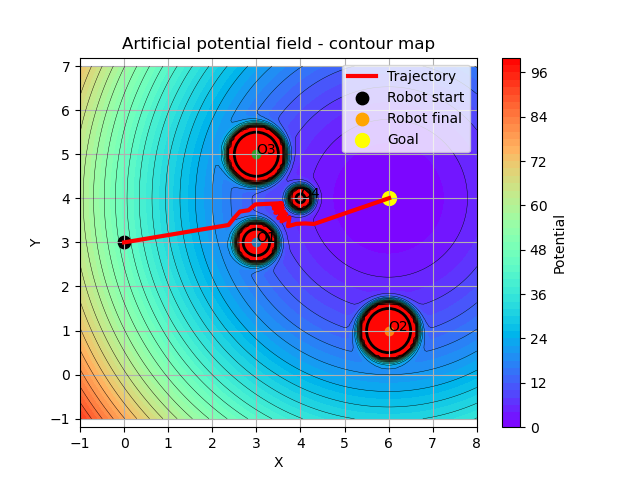
\includegraphics[width=\columnwidth]{Figure_4_2.png}
    \caption{Contour map and robot trajectory for
    $k_{\mathrm{rep}}=5$. The stronger obstacle potentials deform the
    surrounding contours more noticeably.}
    \label{fig:krep_high_contour}
\end{figure}

\begin{figure}[H]
    \centering
    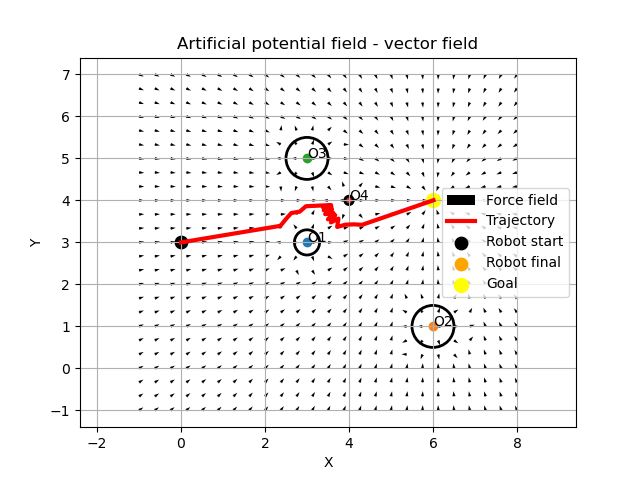
\includegraphics[width=\columnwidth]{Figure_4_3.png}
    \caption{Normalized force field for $k_{\mathrm{rep}}=5$.
    Strong repulsive directions near $O_1$ and $O_4$ produce visible
    oscillations in the robot trajectory.}
    \label{fig:krep_high_vector}
\end{figure}

The experiment shows that a larger repulsive gain increases the safety
response near obstacles, but an excessively large value can produce
sharp deviations, oscillations, or unnecessarily long trajectories.

\[
\begin{aligned}
    k_{\mathrm{rep}}\ \text{large}
    &\Rightarrow
    \text{stronger obstacle avoidance}\\
    &\phantom{\Rightarrow}
    \text{and larger path deviations}.
\end{aligned}
\]

\subsection{Influence of the Repulsive Influence Distance}

The parameter $\rho_0$ defines the maximum clearance at which an
obstacle generates a repulsive contribution:

\begin{equation}
    \mathbf{F}_{\mathrm{rep},i}
    =
    \mathbf{0},
    \qquad
    d_i > \rho_0.
\end{equation}

Since $d_i$ is measured from the obstacle boundary, the effective
influence radius measured from its center is

\begin{equation}
    R_{\mathrm{influence},i}
    =
    r_i+\rho_0.
\end{equation}

Therefore, $\rho_0$ mainly controls the spatial extent of obstacle
avoidance. It also appears inside the repulsive-force expression and
therefore modifies the force profile within the active region.

\subsubsection{Small Influence Distance}

For

\[
    \rho_0=0.1,
\]

the repulsive force becomes active only when the robot is very close to
an obstacle boundary. Most of the workspace is therefore dominated by
the attractive force, and the robot follows an almost direct trajectory
toward the goal.

This produces a short and smooth path, but the robot reacts late to
obstacles and may pass dangerously close to their boundaries.

\begin{figure}[H]
    \centering
    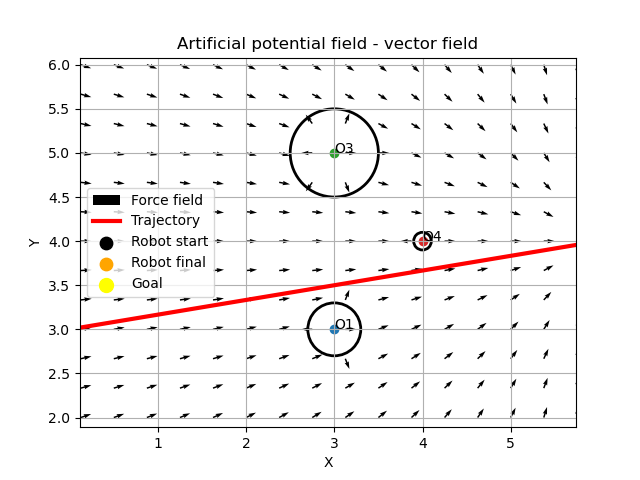
\includegraphics[width=0.95\columnwidth]{Figure_6_3.png}
    \caption{Normalized force field for a small influence distance,
    $\rho_0=0.1$. The obstacles affect only a narrow surrounding region,
    producing an almost direct trajectory toward the goal.}
    \label{fig:rho_small}
\end{figure}

\FloatBarrier

\subsubsection{Large Influence Distance}

For

\[
    \rho_0=10,
\]

the obstacles influence almost the entire workspace. Repulsive
contributions from several obstacles are therefore active
simultaneously, even when the robot is far from their surfaces.

The resulting force field contains stronger directional distortions,
and the trajectory shows visible oscillations and larger deviations.
An excessively large value of $\rho_0$ can therefore make obstacle
avoidance unnecessarily conservative and reduce progress toward the
goal.

\begin{figure}[H]
    \centering
    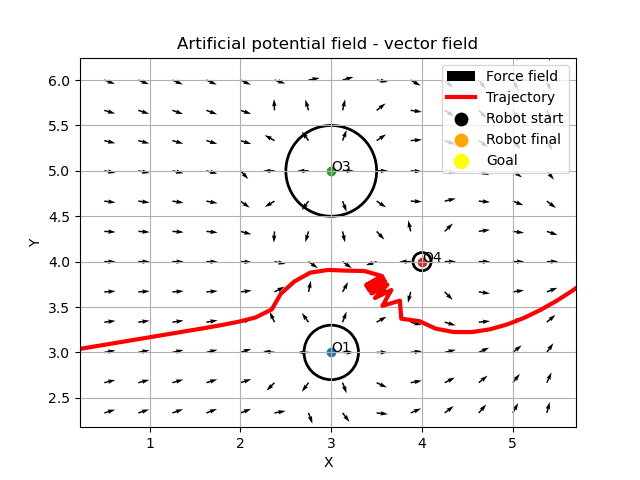
\includegraphics[width=0.95\columnwidth]{Figure_5_3.png}
    \caption{Normalized force field for a large influence distance,
    $\rho_0=10$. Multiple obstacles affect the robot simultaneously,
    producing stronger deviations and oscillations.}
    \label{fig:rho_large}
\end{figure}

\FloatBarrier

The influence of $\rho_0$ can be summarized as

\[
\begin{aligned}
    \rho_0\ \text{small}
    &\Rightarrow
    \text{late obstacle reaction},\\
    \rho_0\ \text{large}
    &\Rightarrow
    \text{wide and potentially excessive repulsion}.
\end{aligned}
\]

A suitable value should provide enough distance for safe obstacle
avoidance without allowing distant obstacles to dominate the navigation
field.

\section{Conclusion}

The experiment demonstrates how an attractive goal and circular obstacles
can be combined within a single reactive navigation framework. The
quadratic attractive potential creates a smooth goal-centered basin, while
the finite-range repulsive potentials generate localized barriers around
the obstacles. The negative gradient of the total potential provides the
robot with a local motion direction without requiring the computation of a
complete global path.

The three visualizations provide complementary interpretations of the same
navigation process. The three-dimensional surface represents the artificial
energy landscape, the contour map shows its spatial distribution, and the
vector field indicates the local direction of motion. The resulting
trajectory emerges from repeatedly following the normalized total force.

The parameter study shows that the behavior of the method depends strongly
on the balance between attraction and repulsion. A small
$k_{\mathrm{att}}$ increases the relative influence of obstacles and may
produce larger deviations or oscillations, whereas a large
$k_{\mathrm{att}}$ produces a more direct trajectory but can weaken the
obstacle-avoidance effect. Increasing $k_{\mathrm{rep}}$ strengthens the
reaction near obstacles without changing the size of their influence
regions. In contrast, $\rho_0$ directly determines how far from an obstacle
the repulsive force becomes active.

The experiment also highlights an important difference between the
potential-field equations and the numerical motion rule. Although the
quadratic attractive force naturally decreases near the goal, normalizing
the total force removes its magnitude information. With a fixed value of
$v\Delta t$, the robot therefore moves using an approximately constant step
length whenever the total force is nonzero. This can produce oscillations
near obstacles or around the goal and may prevent a very small goal
tolerance from being reached.

Artificial potential fields provide a simple and computationally efficient
reactive navigation method. However, they rely only on local information
and can suffer from local minima, oscillations, and excessive sensitivity
to parameter selection. These limitations motivate later extensions such
as adaptive step sizes, mixed attractive potentials, escape behaviors, or
the combination of local potential fields with global path planning.


\section{Project Task}

Represent a mobile robot, one goal, and several circular obstacles in a
two-dimensional workspace. Implement a quadratic attractive potential and
a finite-range repulsive potential based on obstacle clearance. Derive the
corresponding attractive and repulsive forces, sum all force contributions,
normalize the total force, and update the robot position iteratively.

Stop the simulation when the robot enters a specified goal tolerance or
when a maximum number of steps is reached. Visualize the total potential as
a three-dimensional surface and contour map, draw the normalized force
field, and overlay the resulting robot trajectory.

Finally, study the influence of the attractive gain
$k_{\mathrm{att}}$, the repulsive gain $k_{\mathrm{rep}}$, and the
repulsive influence distance $\rho_0$. Compare the quadratic attractive
formulation with the conic model and explain how a mixed potential can
combine bounded far-field attraction with smooth near-goal convergence.

% =================================================
\end{document}
% =================================================
